\documentclass[11pt,a4paper]{article}

\usepackage[utf8]{inputenc}
\usepackage[T1]{fontenc}
\usepackage[margin=2.2cm]{geometry}
\usepackage{amsmath}
\usepackage{textcomp}
\usepackage{graphicx}
\usepackage{booktabs}
\usepackage{array}
\usepackage{caption}
\usepackage{xcolor}
\usepackage{hyperref}
\hypersetup{colorlinks=true,linkcolor=blue!50!black,urlcolor=blue!50!black,citecolor=blue!50!black}
\captionsetup{font=small,labelfont=bf}

\newcommand{\glmdir}{../analysis/05-glm}
\newcommand{\badir}{../analysis/04-block-average}
\newcommand{\roiview}[1]{\includegraphics[width=0.235\textwidth,trim=90 150 90 150,clip]{../analysis/00-rois/#1_head_800x800_transparent.png}}
\newcommand{\baframe}[3]{\includegraphics[width=0.22\textwidth,trim=60 130 60 150,clip]{\badir/#1-movies/#2_blockavg_frames/left/frame_#3.png}}

\title{Piano playing in quiet and in pink noise:\\ a single-subject fNIRS pilot
(LYDIA)}
\author{Adam Emile Aske}
\date{2026-09-23}

\begin{document}
\maketitle

\section{Methods}


\subsection{Participant, task and sessions}
A student pianist (sub-01, graduate level) played Gymnopédie no.~1 (Erik
Satie) on a piano in a music recording studio hall. In the NOISE condition a
loudspeaker placed behind and to the left of the player emitted pink noise. In
QUIET the room was silent. Sessions were run in the order \texttt{quiet\_1}
(ses-08),
\texttt{noise\_1} (ses-09), \texttt{quiet\_2} (ses-10), \texttt{noise\_2}
(ses-11), all on 2026-09-07. Each session was one run of 6 play blocks
(planned $40\pm8$\,s, jittered) separated by rest ($30\pm5$\,s), preceded by a
60\,s baseline. A 1\,kHz beep cued each play (1 beep) and rest (2 beeps)
onset. Markers were sent over the Lab Streaming Layer (LSL) with codes 20 =
play(QUIET), 21 = play(NOISE) and 30 = rest. Executed play blocks lasted
32--46\,s (mean 38.4\,s, \texttt{data/blocks.csv}); the design of the four
runs is shown in Fig.~\ref{fig:design}.

\begin{figure}[htbp]
\centering
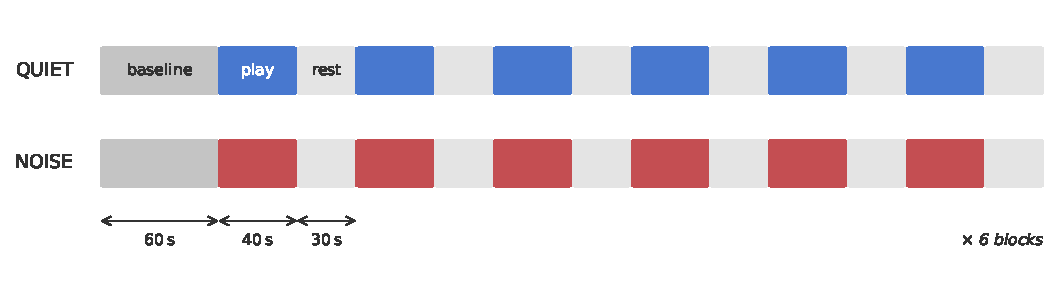
\includegraphics[width=0.92\textwidth]{figures/block_design.pdf}
\caption{Block design (schematic). Each run began with a 60\,s baseline and
alternated 6 play blocks with rest; the QUIET and NOISE runs share the same
structure. Play and rest durations were jittered around the nominal 40 and
30\,s shown here (executed play blocks 32--46\,s), and the GLM modelled every
block as a 40\,s boxcar.}
\label{fig:design}
\end{figure}

\subsection{Montage and acquisition}
Functional near-infrared spectroscopy (fNIRS) data were acquired with a
NIRSport2 (Aurora 2025.2) at 760/850\,nm and 12.2\,Hz. The optode layout
(Fig.~\ref{fig:montage}) uses 16 sources and 16 detectors on EEG 10-10 sites,
giving 47 channels of 30--42\,mm separation (mean 35.4\,mm). Coverage: frontal
pole and ventrolateral prefrontal cortex (VLPFC; Fpz, AF7, AF8 $\rightarrow$
Fp1, Fp2, AFz), dorsolateral prefrontal cortex (DLPFC) (AF3, AF4, Fz, F3, F4
$\rightarrow$ F5, F1, F2, F6), premotor and supplementary motor area (SMA;
FC5, FC1, FC2, FC6 $\rightarrow$ FC3, FCz, FC4), sensorimotor (C3, C4
$\rightarrow$ C5, C6) and temporal (T7, T8 $\rightarrow$ FT7, TP7, FT8, TP8).

\begin{figure}[htbp]
\centering
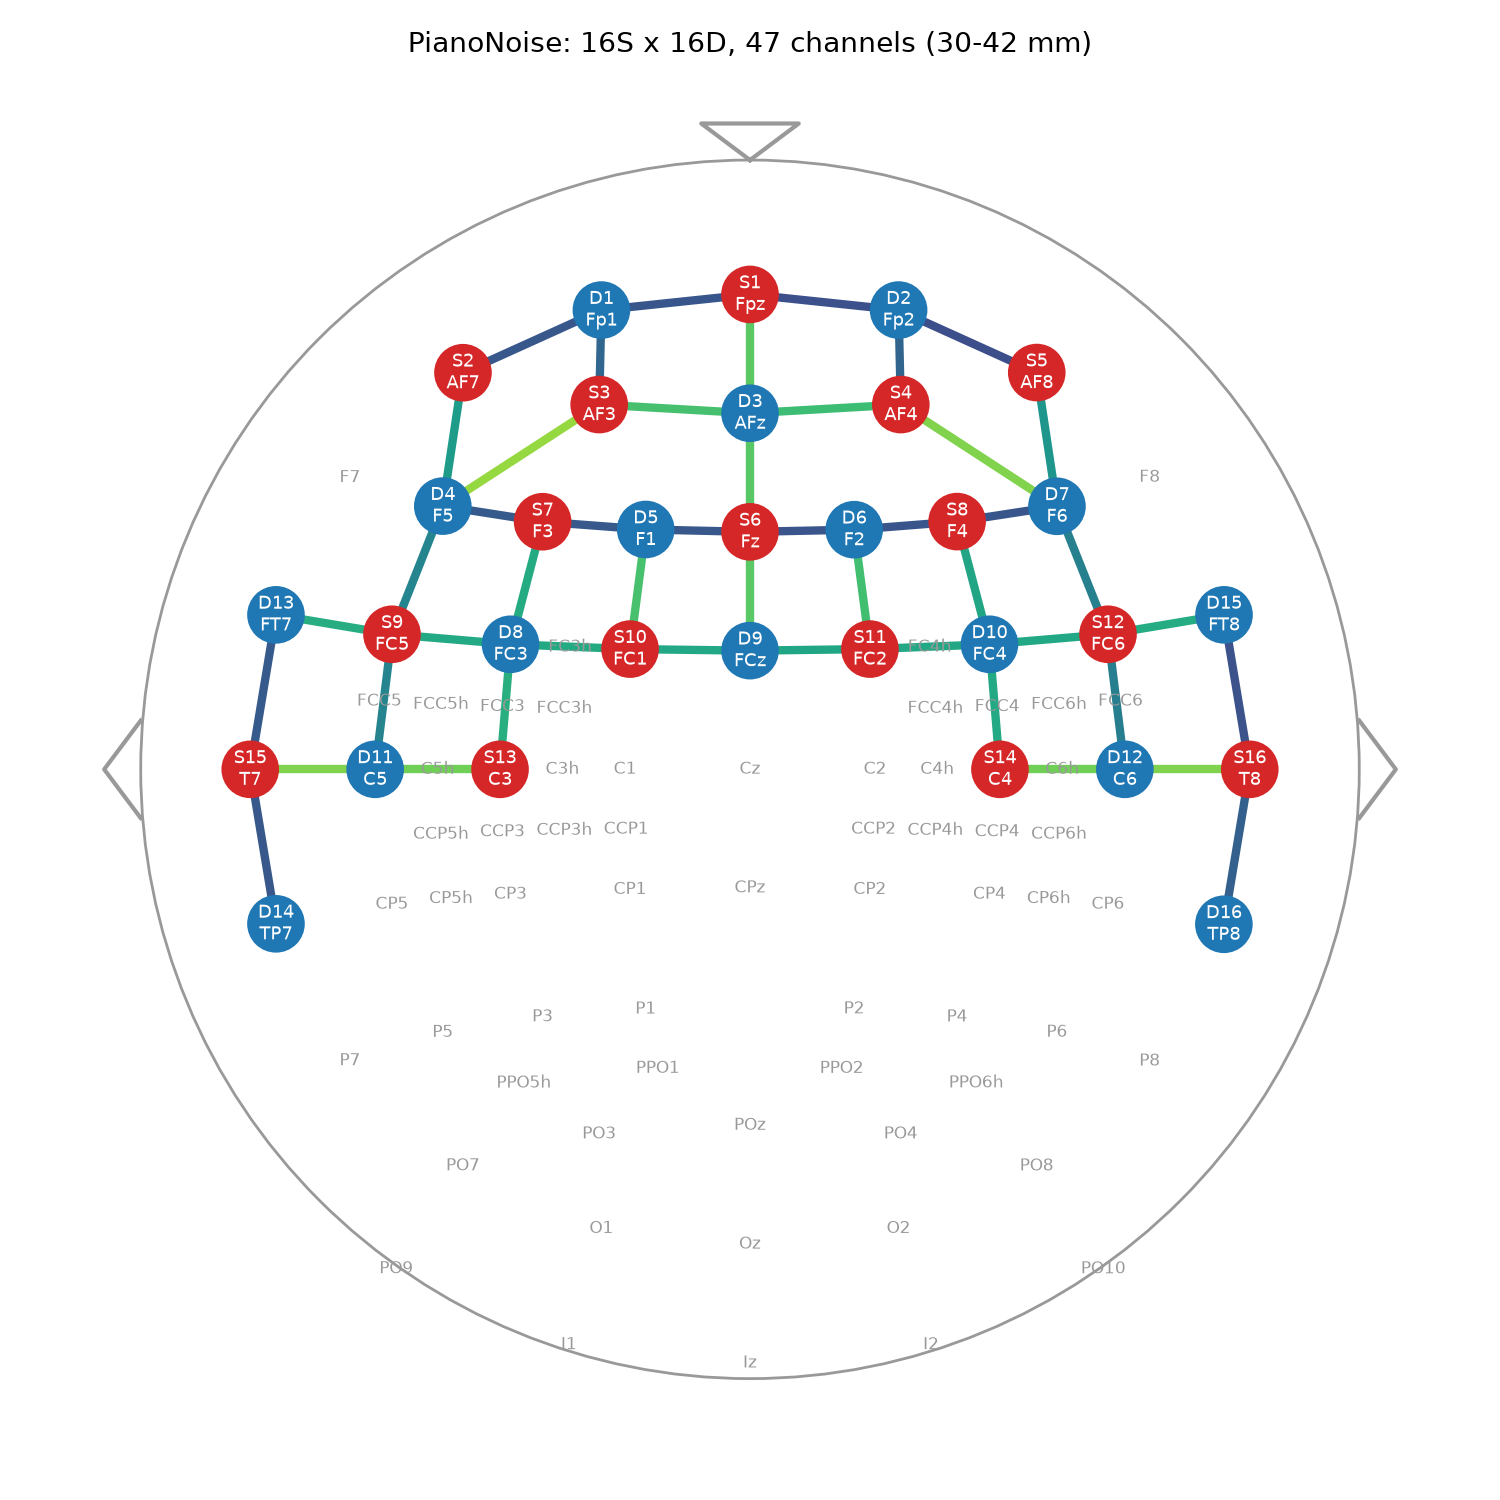
\includegraphics[width=0.62\textwidth]{figures/montage_2d.png}
\caption{The optode layout, top view (nose up). Red: sources
S1--S16, blue: detectors D1--D16, lines: the 47 channels (colour =
source--detector distance, 30--42\,mm).}
\label{fig:montage}
\end{figure}

\subsection{Quality control}
Signal quality was assessed per run in NIRWizard 0.2.1 in non-overlapping 5\,s
windows using the scalp coupling index (SCI, cardiac band 0.5--2.5\,Hz) and
peak spectral power (PSP). A window was good when SCI $\geq 0.8$ and PSP
$\geq 0.1$, and a channel was good when at least 75\,\% of its windows were
good and SNR $\geq 2$. The census is reported descriptively
(Table~\ref{tab:qc}); no channels were excluded, and all 47 channels enter the
analyses below.

\subsection{Regions of interest}
Ten regions of interest (ROIs) were defined in NIRWizard as five left/right
pairs: VLPFC, DLPFC, temporal, premotor (PMA) and SMA
(Fig.~\ref{fig:rois}, Table~\ref{tab:ba}). Some channels belong to two ROIs
(e.g.\ S1-D3 and S6-D3 to both DLPFC ROIs, S6-D9 to both SMA ROIs, S9-D4 to
left VLPFC and left PMA, S12-D7 to right VLPFC and right PMA).

\begin{figure}[htbp]
\centering
\begin{tabular}{@{}c@{}c@{}c@{}c@{}}
\roiview{left} & \roiview{right} & \roiview{anterior} & \roiview{superior}
\end{tabular}
\caption{The ten ROIs on the cortex (left, right, anterior, superior view).}
\label{fig:rois}
\end{figure}

\subsection{Preprocessing}
Preprocessing was done in NIRWizard 0.2.1 (cedalion 26.5.1 backend):
(1) conversion of raw intensity to optical density; (2) motion correction in
three stages, recursive PCA (9 artefact segments, 15 components removed),
temporal derivative distribution repair (TDDR) and wavelet correction (db2,
level 4, IQR 1.5); (3) zero-phase Butterworth band-pass 0.01--0.2\,Hz;
(4) modified Beer--Lambert law with age-dependent differential pathlength
factors (assumed age 25) to $\Delta$HbO and $\Delta$HbR in \textmu M. The
montage has no short-separation channels (all separations $\geq 30$\,mm), so
no short-channel regression was applied and scalp and systemic signals remain
in the data.

\subsection{Analysis}
\paragraph{Block averages.} Computed per run. Epochs of $-10$ to 50\,s around
each play onset were baseline-corrected by the mean of the $-10$ to 0\,s window
and averaged over the 12 blocks per condition (6 per run, no epoch rejection).
ROI curves are the mean over the channels of each ROI.

\paragraph{GLM.} For the GLM the four raw recordings were first concatenated
into a single session (26\,159 samples) and then preprocessed together with the
pipeline above, so that motion correction, filtering and the concentration
conversion act on one coherent signal rather than on four separately scaled
ones. The design held one regressor per condition (12 blocks each, 40\,s boxcar
convolved with the canonical SPM HRF) with its temporal derivative as
nuisance, an intercept and three run intercepts. It was fitted per channel and
chromophore with AR-IRLS: BIC-selected autoregressive prewhitening, pooled over
the session and restarted at each run boundary, with robust iterative
reweighting. Each condition is tested against the rest baseline.
$p$-values were corrected with Benjamini--Hochberg FDR across channels within
condition $\times$ chromophore (residual degrees of freedom 26\,151). Maps are
shown unthresholded and thresholded, at $|t|>20$ for HbO and, because the HbR
response is smaller, at $|t|>10$ for HbR.

\paragraph{Laterality.} The Seghier index $\mathrm{LI} = (L-R)/(|L|+|R|)$ was
computed per ROI pair from the ROI mean GLM $\beta$ (and $t$), with
$|\mathrm{LI}| > 0.2$ read as lateralised. LI is interpretable when both sides
are positive.

\section{Results}

\subsection{Quality control}
\begin{table}[htbp]
\centering\small
\begin{tabular}{lrrrrr}
\toprule
Run & Duration (s) & Bad / 47 & SCI fail & PSP fail & GVTD median \\
\midrule
quiet\_1 & 622 & 28 & 11 & 26 & 0.0095 \\
noise\_1 & 516 & 26 & 13 & 24 & 0.0099 \\
quiet\_2 & 498 & 23 & 13 & 22 & 0.0104 \\
noise\_2 & 507 & 29 & 11 & 27 & 0.0107 \\
\bottomrule
\end{tabular}

\caption{Per-run QC census. GVTD: global variance of the temporal derivative.}
\label{tab:qc}
\end{table}

Between 23 and 29 of 47 channels fell below the PSP criterion in each run,
while SNR never failed and GVTD was low and stable across runs (medians
0.0095--0.0107), so the recordings are clean of motion but the cardiac
signal is weak in part of the montage. The weaker channels lie over the
premotor, lateral SMA and temporal optodes (S7--S15), consistent with hair;
prefrontal channels were good throughout. Results from the PMA and SMA ROIs
should be read with this in mind.

\subsection{Block averages}
\begin{figure}[htbp]
\centering
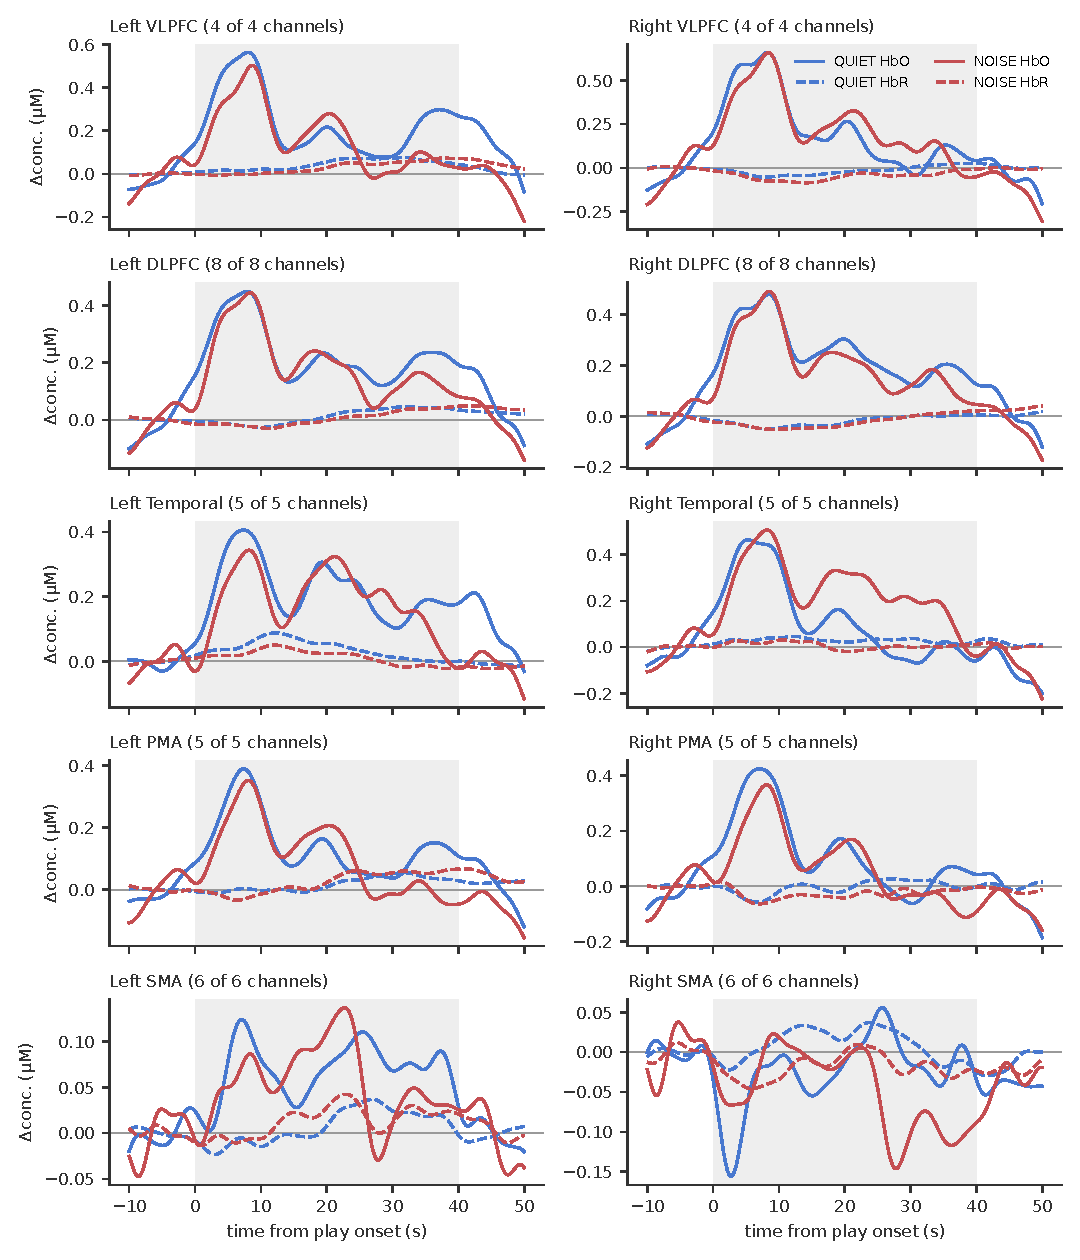
\includegraphics[width=\textwidth]{figures/ba_roi.pdf}
\caption{ROI block averages (12 blocks per condition). Solid: HbO, dashed:
HbR. Grey: nominal 40\,s play block. Note the different $y$ scales.}
\label{fig:ba}
\end{figure}

\begin{table}[htbp]
\centering\small
\begin{tabular}{llrrrr}
\toprule
ROI & Ch. & QUIET HbO & QUIET HbR & NOISE HbO & NOISE HbR \\
\midrule
Left VLPFC & 4/4 & 0.230 & 0.048 & 0.165 & 0.034 \\
Right VLPFC & 4/4 & 0.197 & -0.016 & 0.229 & -0.049 \\
Left DLPFC & 8/8 & 0.226 & 0.016 & 0.194 & 0.007 \\
Right DLPFC & 8/8 & 0.245 & -0.019 & 0.208 & -0.021 \\
Left Temporal & 5/5 & 0.224 & 0.038 & 0.200 & 0.013 \\
Right Temporal & 5/5 & 0.103 & 0.029 & 0.252 & 0.006 \\
Left PMA & 5/5 & 0.140 & 0.021 & 0.108 & 0.028 \\
Right PMA & 5/5 & 0.114 & -0.001 & 0.076 & -0.030 \\
Left SMA & 6/6 & 0.077 & 0.011 & 0.059 & 0.016 \\
Right SMA & 6/6 & -0.013 & 0.014 & -0.048 & -0.018 \\
\bottomrule
\end{tabular}

\caption{Mean block-averaged concentration change 5--40\,s after play onset
(\textmu M). Ch.: channels in the ROI.}
\label{tab:ba}
\end{table}

\begin{figure}[htbp]
\centering
\begin{tabular}{@{}r@{\,}c@{}c@{}c@{}c@{}}
 & 0\,s & 8\,s & 20\,s & 40\,s \\
\rotatebox{90}{\small QUIET HbO} & \baframe{hbo}{QUIET}{00122} & \baframe{hbo}{QUIET}{00220} & \baframe{hbo}{QUIET}{00366} & \baframe{hbo}{QUIET}{00610} \\
\rotatebox{90}{\small NOISE HbO} & \baframe{hbo}{NOISE}{00122} & \baframe{hbo}{NOISE}{00220} & \baframe{hbo}{NOISE}{00366} & \baframe{hbo}{NOISE}{00610} \\
\rotatebox{90}{\small QUIET HbR} & \baframe{hbr}{QUIET}{00122} & \baframe{hbr}{QUIET}{00220} & \baframe{hbr}{QUIET}{00366} & \baframe{hbr}{QUIET}{00610} \\
\rotatebox{90}{\small NOISE HbR} & \baframe{hbr}{NOISE}{00122} & \baframe{hbr}{NOISE}{00220} & \baframe{hbr}{NOISE}{00366} & \baframe{hbr}{NOISE}{00610} \\
\end{tabular}
\caption{Block-averaged $\Delta$HbO (top two rows) and $\Delta$HbR (bottom two
rows) on the cortex, left view, at four times after play onset. Frames from
the movies in \texttt{analysis/04-block-average/hbo-movies} and
\texttt{hbr-movies}.}
\label{fig:frames}
\end{figure}

In both conditions HbO rose at play onset in the prefrontal, temporal and
premotor ROIs, peaked 7--9\,s after onset, fell back to roughly a third of
the peak by 15\,s and stayed slightly elevated to the end of the block
(Fig.~\ref{fig:ba}, Fig.~\ref{fig:frames}). The response is an onset transient
followed by a low plateau. HbR changed little (within about
$\pm 0.05$\,\textmu M) and did not show the decrease that accompanies a typical
neurovascular response; in the left-hemisphere ROIs it rose slightly. The
time course has nearly the same shape in every prefrontal and temporal ROI,
which suggests a systemic contribution alongside cortical activation. The SMA
ROIs showed small responses ($<0.15$\,\textmu M). The QUIET and NOISE curves
largely overlap; the plateau was higher in NOISE in the right temporal ROI
(0.25 vs 0.10\,\textmu M) and higher in QUIET in left VLPFC (0.23 vs
0.17\,\textmu M).

\subsection{GLM}
\begin{table}[htbp]
\centering\small
\begin{tabular}{llrrrrr}
\toprule
Condition & Signal & $q<.05$, $t>0$ & $q<.05$, $t<0$ & $|t|>20$ & median $\beta$ & $t$ range \\
\midrule
QUIET & HbO & 45 & 1 & 15 & 0.131 & -2.9 to 45.0 \\
QUIET & HbR & 25 & 16 & 2 & 0.004 & -22.3 to 20.9 \\
NOISE & HbO & 42 & 2 & 11 & 0.108 & -17.7 to 37.8 \\
NOISE & HbR & 21 & 18 & 3 & 0.000 & -25.3 to 23.2 \\
\bottomrule
\end{tabular}

\caption{Channel-level GLM results over the 47 channels: number of channels
with FDR $q<0.05$ by sign, number with $|t|>20$, median $\beta$ (\textmu M)
and range of $t$.}
\label{tab:census}
\end{table}

\begin{figure}[p]
\centering
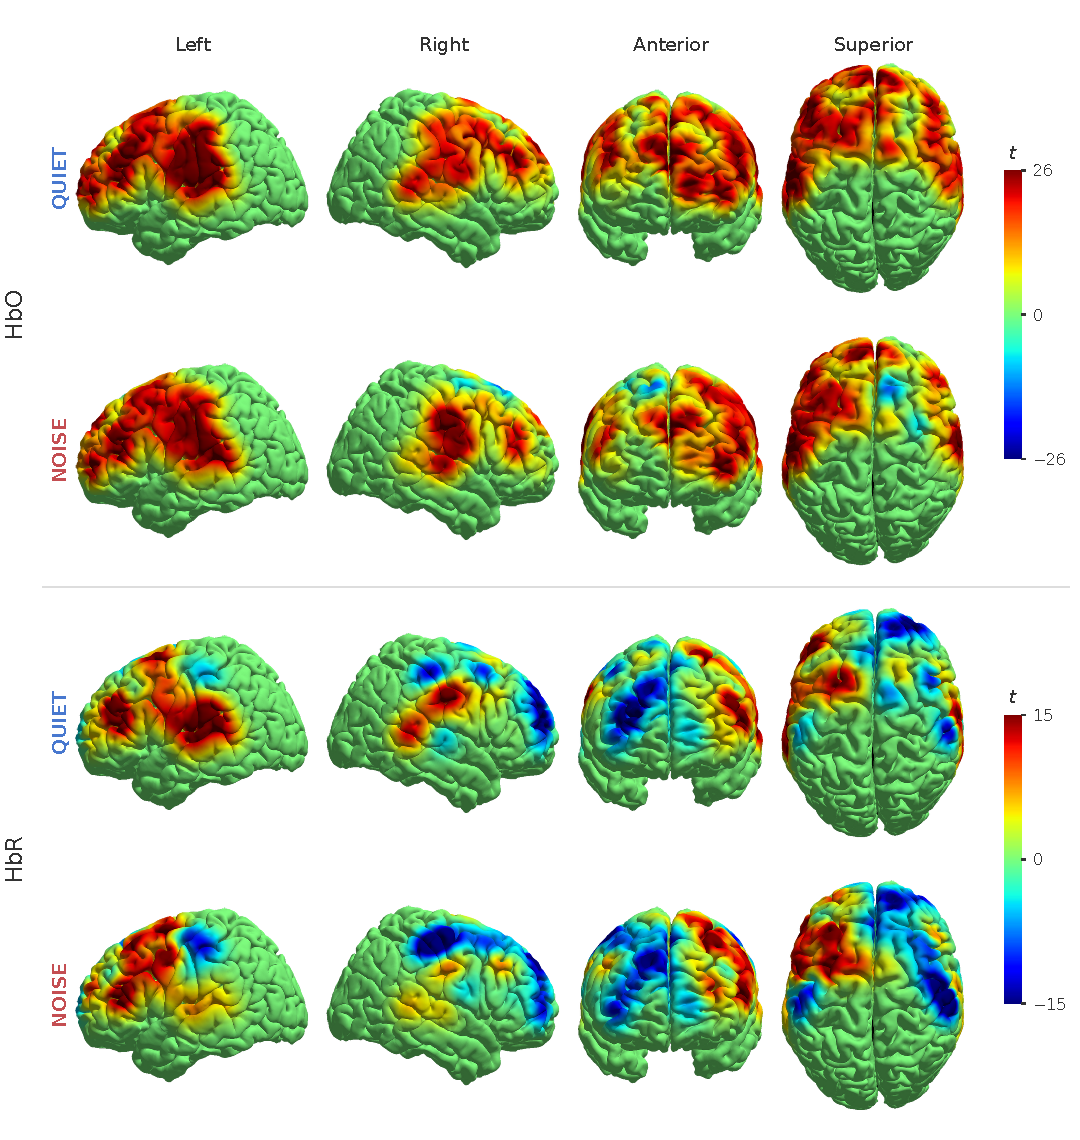
\includegraphics[width=\textwidth]{figures/glm_maps_unthresholded.pdf}
\caption{GLM $t$ maps on the cortex, unthresholded, for HbO (colour scale
$\pm 26$) and HbR ($\pm 15$). For HbR, positive $t$ is an increase.}
\label{fig:glmall}
\end{figure}

\begin{figure}[p]
\centering
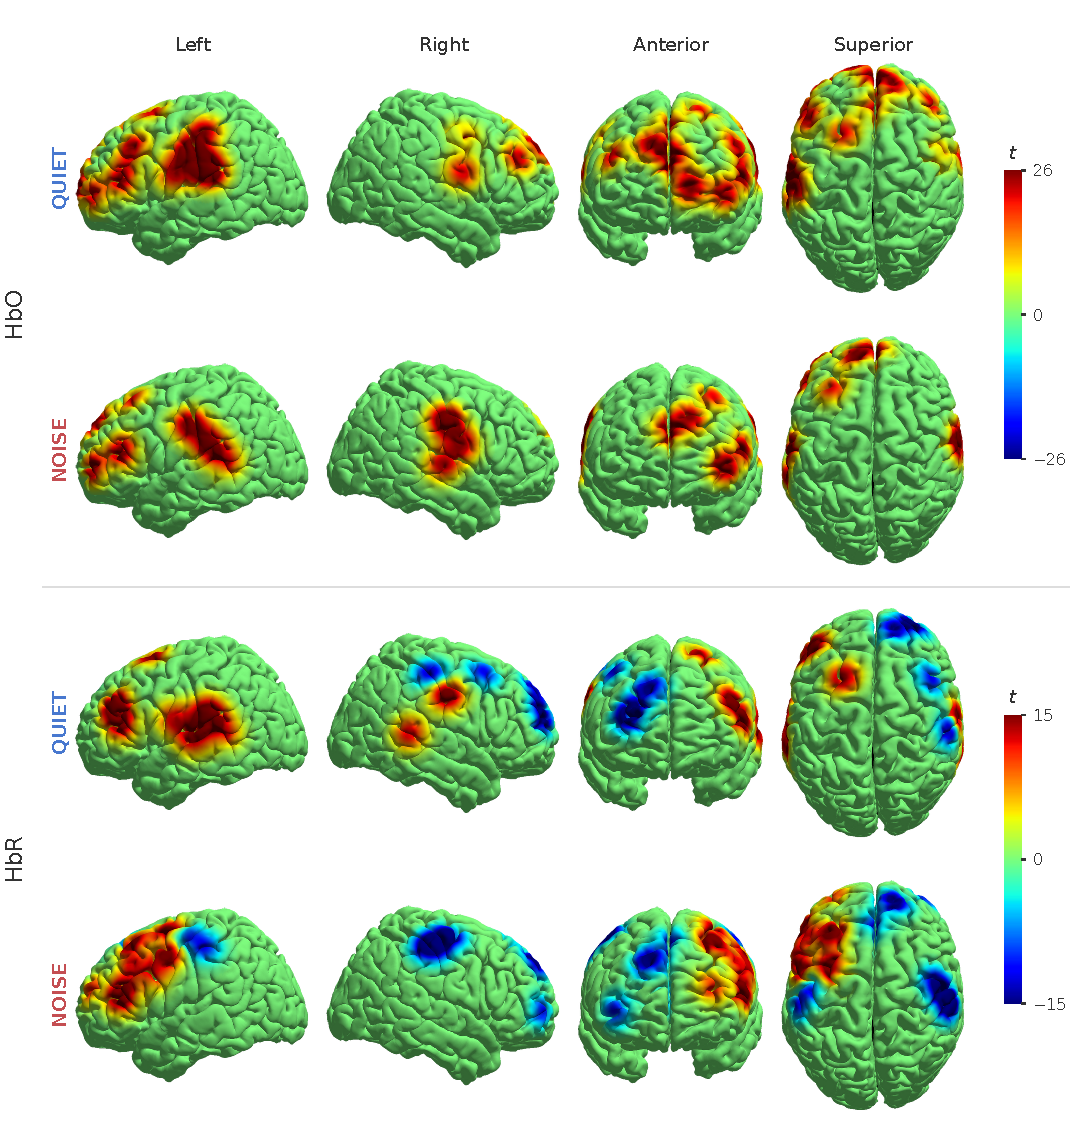
\includegraphics[width=\textwidth]{figures/glm_maps_thresholded.pdf}
\caption{GLM $t$ maps thresholded at $|t|>20$ for HbO and $|t|>10$ for HbR,
layout and colour scales as Fig.~\ref{fig:glmall}.}
\label{fig:glmthr}
\end{figure}

\begin{table}[htbp]
\centering\small
\begin{tabular}{@{}c@{}}
\hspace{2.6cm}QUIET HbO\hspace{0.9cm}NOISE HbO\hspace{0.9cm}QUIET HbR\hspace{0.9cm}NOISE HbR\\
\begin{tabular}{lr rrrr rrrr}
\toprule
ROI & $n$ & $\beta$ & $t$ & $\beta$ & $t$ & $\beta$ & $t$ & $\beta$ & $t$ \\
\midrule
Left VLPFC & 4 & 0.229 & 20.7 & 0.261 & 23.4 & 0.023 & 12.8 & 0.016 & 7.6 \\
Right VLPFC & 4 & 0.111 & 11.0 & 0.104 & 9.9 & 0.002 & 1.6 & -0.005 & -1.7 \\
Left DLPFC & 8 & 0.195 & 21.4 & 0.140 & 16.4 & -0.004 & -2.4 & 0.001 & 2.3 \\
Right DLPFC & 8 & 0.182 & 17.7 & 0.092 & 8.0 & -0.014 & -7.5 & -0.014 & -8.7 \\
Left Temporal & 5 & 0.181 & 25.6 & 0.170 & 23.0 & 0.029 & 12.9 & 0.010 & 3.3 \\
Right Temporal & 5 & 0.146 & 16.5 & 0.163 & 19.5 & 0.022 & 6.9 & 0.010 & 3.1 \\
Left PMA & 5 & 0.100 & 14.5 & 0.117 & 16.9 & 0.008 & 3.0 & 0.003 & 0.9 \\
Right PMA & 5 & 0.153 & 17.6 & 0.079 & 9.0 & -0.009 & -2.3 & -0.035 & -9.7 \\
Left SMA & 6 & 0.067 & 11.9 & 0.057 & 10.7 & 0.008 & 3.7 & 0.017 & 10.2 \\
Right SMA & 6 & 0.041 & 6.9 & -0.018 & -2.6 & 0.001 & -0.2 & -0.002 & -1.0 \\
\bottomrule
\end{tabular}

\end{tabular}
\caption{ROI mean GLM $\beta$ (\textmu M) and mean $t$ over the $n$ channels
of each ROI.}
\label{tab:glmroi}
\end{table}

HbO $\beta$ was positive and significant in 45 of 47 channels for QUIET and
42 of 47 for NOISE (Table~\ref{tab:census}, Fig.~\ref{fig:glmall}). At
$|t|>20$ (Fig.~\ref{fig:glmthr}), 15 channels remained in QUIET and 11 in NOISE. In QUIET these
were left temporal (S15-D11, $t=45$; S9-D11, S9-D13), medial and left DLPFC
(S1-D3, S1-D1, S6-D3, S7-D4), left VLPFC (S2-D1, S2-D4), right DLPFC (S4-D3,
S4-D7) and single premotor and right temporal channels. In NOISE the
left VLPFC, left temporal and medial DLPFC channels were again the strongest,
joined by right temporal (S12-D12, $t=38$; S12-D15, S16-D15), while the
right DLPFC channels dropped below the threshold. By ROI
(Table~\ref{tab:glmroi}), responses were largest in left VLPFC
(0.23 and 0.26\,\textmu M in QUIET and NOISE), DLPFC and the temporal ROIs
and smallest in the SMA. The right-hemisphere DLPFC and PMA responses were
about half as large in NOISE as in QUIET (DLPFC 0.18 vs 0.09, PMA 0.15 vs
0.08\,\textmu M), whereas the left-hemisphere and temporal responses were
similar in the two conditions.

HbR $\beta$ was an order of magnitude smaller, centred on zero, and
significant in both directions in similar numbers of channels
(Fig.~\ref{fig:glmall}, bottom rows); 13 channels in QUIET and 15 in NOISE
exceeded $|t|>10$ (Fig.~\ref{fig:glmthr}). It increased in left VLPFC and the temporal ROIs and
decreased in right DLPFC and, in NOISE, right PMA; the HbO-up, HbR-down
pattern of a typical haemodynamic response was thus clearest in right DLPFC.
The $t$ values are large because the fit has 26\,151 residual degrees of
freedom from one person's 12\,Hz samples: they express how consistently the
signal follows the block timing within this session.

\subsection{Laterality}
\begin{figure}[htbp]
\centering
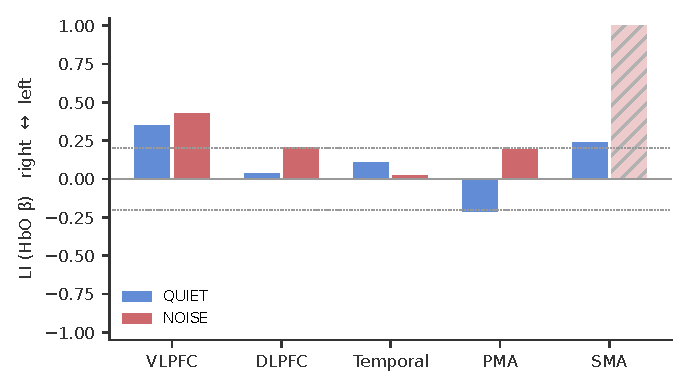
\includegraphics[width=0.62\textwidth]{figures/laterality.pdf}
\caption{Laterality index of the HbO GLM $\beta$ per ROI pair. Dotted lines:
$\pm 0.2$. Hatched: left and right have opposite signs, so $|\mathrm{LI}|=1$
regardless of magnitude.}
\label{fig:li}
\end{figure}

HbO responses were left-dominant overall (whole-hemisphere LI 0.10 in QUIET,
0.29 in NOISE; Fig.~\ref{fig:li}). VLPFC was left-lateralised in both
conditions (0.35 and 0.43). DLPFC was bilateral in QUIET (0.03) and
left-lateralised in NOISE (0.21), because the right-hemisphere response was
smaller in NOISE while the left changed less. The temporal ROIs were
bilateral in both conditions (0.11, 0.02). PMA was right-lateralised in QUIET
($-0.21$) and close to left-lateralised in NOISE (0.19). SMA was
left-lateralised in QUIET (0.24); its value of 1.0 in NOISE reflects a
negative right-SMA $\beta$ and is not a meaningful magnitude. Indices from
$t$ values agree in sign and ordering. HbR indices are not reported: the HbR
amplitudes are near zero and of mixed sign, which makes the ratio unstable.

\section{Discussion}
Piano playing produced a robust HbO increase over prefrontal, temporal and
premotor cortex in both conditions, strongest in left VLPFC, DLPFC and the
temporal ROIs, and left-dominant overall. The response was an onset transient
followed by a low plateau, similar in shape across regions, and HbR did not
decrease outside right DLPFC. This points to a systemic contribution, which
this montage cannot remove because it has no short-separation channels.

The two conditions gave similar maps. Descriptively, the right DLPFC and
right PMA responded less in NOISE, which made the NOISE pattern more
left-lateralised, and the right temporal response was somewhat larger in
NOISE. These are observations in one participant and one session.

\end{document}
